\documentclass[
11pt, % The default document font size, options: 10pt, 11pt, 12pt
%codirector, % Uncomment to add a codirector to the title page
]{charter} 


% El títulos de la memoria, se usa en la carátula y se puede usar el cualquier lugar del documento con el comando \ttitle
\titulo{Pronóstico de ventas para toma de decisiones en comercio electrónico usando \textit{Machine Learning}} 

% Nombre del posgrado, se usa en la carátula y se puede usar el cualquier lugar del documento con el comando \degreename
\posgrado{Carrera de Especialización en Inteligencia Artificial} 
%\posgrado{Carrera de Especialización en Internet de las Cosas} 
%\posgrado{Carrera de Especialización en Inteligencia Artificial}
%\posgrado{Maestría en Sistemas Embebidos} 
%\posgrado{Maestría en Internet de las cosas}

% Tu nombre, se puede usar el cualquier lugar del documento con el comando \authorname
% IMPORTANTE: no omitir titulaciones ni tildación en los nombres, también se recomienda escribir los nombres completos (tal cual los tienen en su documento)
\autor{Ing. Jonathan Matías Borda}

% El nombre del director y co-director, se puede usar el cualquier lugar del documento con el comando \supname y \cosupname y \pertesupname y \pertecosupname
\director{Título y Nombre del director (a confirmar)}
\pertenenciaDirector{pertenencia} 
\codirector{} % para que aparezca en la portada se debe descomentar la opción codirector en los parámetros de documentclass
\pertenenciaCoDirector{FIUBA}

% Nombre del cliente, quien va a aprobar los resultados del proyecto, se puede usar con el comando \clientename y \empclientename
\cliente{Lic. Juan Cruz Bonina}
\empresaCliente{Latech}
 
\fechaINICIO{24 de junio de 2025}		%Fecha de inicio de la cursada de GdP \fechaInicioName
\fechaFINALPlan{12 de agosto de 2025} 	%Fecha de final de cursada de GdP
\fechaFINALTrabajo{27 de julio de 2026}	%Fecha de defensa pública del trabajo final


\begin{document}

\maketitle
\thispagestyle{empty}
\pagebreak


\thispagestyle{empty}
{\setlength{\parskip}{0pt}
\tableofcontents{}
}
\pagebreak


\section*{Registros de cambios}
\label{sec:registro}


\begin{table}[ht]
\label{tab:registro}
\centering
\begin{tabularx}{\linewidth}{@{}|c|X|c|@{}}
\hline
\rowcolor[HTML]{C0C0C0} 
Revisión & \multicolumn{1}{c|}{\cellcolor[HTML]{C0C0C0}Detalles de los cambios realizados} & Fecha      \\ \hline
0      & Creación del documento                                 &\fechaInicioName \\ \hline
1      & Se completa hasta el punto 5 inclusive                & 8 de julio de 2025 \\ \hline
2      & Se completa hasta el punto 9 inclusive                & 15 de julio de 2025 \\ \hline
%		  Se puede agregar algo más \newline
%		  En distintas líneas \newline
%		  Así                                                    & {día} de {mes} de 202X \\ \hline
%3      & Se completa hasta el punto 12 inclusive                & {día} de {mes} de 202X \\ \hline
%4      & Se completa el plan	                                 & {día} de {mes} de 202X \\ \hline

% Si hay más correcciones pasada la versión 4 también se deben especificar acá

\end{tabularx}
\end{table}

\pagebreak



\section*{Acta de constitución del proyecto}
\label{sec:acta}

\begin{flushright}
Buenos Aires, \fechaInicioName
\end{flushright}

\vspace{2cm}

Por medio de la presente se acuerda con el \authorname\hspace{1px} que su Trabajo Final de la \degreename\hspace{1px} se titulará ``\ttitle'' y consistirá en desarrollar un modelo de inteligencia artificial capaz de pronosticar las ventas de una tienda en línea de la empresa \empclientename. El trabajo tendrá un presupuesto preliminar estimado de 684 horas y un costo estimado de \$12.825.000, con fecha de inicio el \fechaInicioName\hspace{1px} y fecha de presentación pública el {\fechaFinalName }.

Se adjunta a esta acta la planificación inicial.

\vfill

% Esta parte se construye sola con la información que hayan cargado en el preámbulo del documento y no debe modificarla
\begin{table}[ht]
\centering
\begin{tabular}{ccc}
\begin{tabular}[c]{@{}c@{}}Dr. Ing. Ariel Lutenberg \\ Director posgrado FIUBA\end{tabular} & \hspace{2cm} & \begin{tabular}[c]{@{}c@{}}\clientename \\ \empclientename \end{tabular} \vspace{2.5cm} \\ 
\multicolumn{3}{c}{\begin{tabular}[c]{@{}c@{}} \supname \\ Director del Trabajo Final\end{tabular}} \vspace{2.5cm} \\
\end{tabular}
\end{table}




\section{1. Descripción técnica-conceptual del proyecto a realizar}
\label{sec:descripcion}

La empresa \empclientename\ fabrica y comercializa barritas alimenticias en distintos sabores. 
Como se trata de alimentos, la empresa necesita contar con pronósticos precisos de ventas, que le permitan planificar la producción y evitar tanto faltantes como excedentes de stock.

A partir de esta problemática, se propone desarrollar un modelo de inteligencia artificial capaz de pronosticar las ventas de la tienda en línea de la empresa \empclientename. 

El desafío es que la precisión de la predicción de las ventas sea alta para que el cliente pueda tomar decisiones estratégicas con un alto grado de confianza. 
A su vez, el cliente desea conocer la evolución de las ventas en el tiempo para poder ajustar la estrategia de marketing y de ventas en función de los resultados.

Se va a utilizar como insumo un conjunto de datos históricos, que abarca aproximadamente dos años, sobre ventas e inversión en publicidad. 
Estos datos se van a obtener desde Shopify, la plataforma donde el cliente tiene alojada su tienda, con el propósito final de contar con una herramienta que facilite la toma de decisión estratégica basada en la predicción.

La plataforma Shopify está basada en la nube y permita a empresas y particulares crear y gestionar tiendas en línea. 
Además, esta ofrece una \textit{API} que facilita el acceso a datos como: los productos vendidos por día, los usuarios que realizan la compra, el canal de venta, etc. 
A través de esta \textit{API} también se obtienen métricas de comportamiento de los usuarios tales como: la cantidad de páginas vistas, cuando agrega un producto al carrito de compra, cuando termina la compra y la tasa de conversión.
Adicionalmente, se utiliza una plataforma llamada Triple Whale, especializada en la gestión y análisis de inversión publicitaria que proporciona una \textit{API} donde se obtiene información sobre la inversión realizada por la tienda en sitios como: Google, Facebook, Instagram, Klaviyo,etc.

Para llevar a cabo el proyecto se cuenta con el financiamiento de la empresa \empclientename\ y acceso a la \textit{API} de Shopify y a la \textit{API} de Triple Whale. 
Asimismo, existe un acuerdo de confidencialidad con la empresa, que establece que los datos utilizados y los entregables generados durante el desarrollo del proyecto no podrán ser difundidos públicamente ni compartidos con terceros sin autorización expresa.

En la figura \ref{fig:diagBloques} se presenta el diagrama en bloques del sistema. Se observa que las \textit{APIs} externas proveen los datos que alimentan el conjunto de datos del proyecto. Tanto este conjunto de datos como el modelo de predicción se integrarán dentro del sistema del cliente, denominado Inventory Tracker. Como resultado, el sistema generará el pronóstico de ventas.

\begin{figure}[htpb]
\centering 
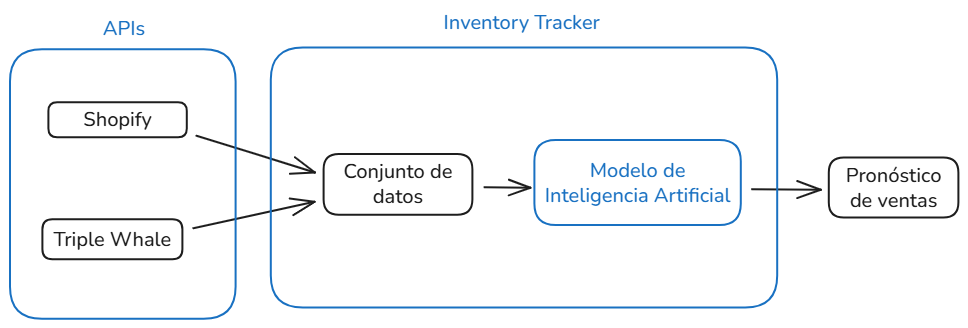
\includegraphics[width=1\textwidth]{./Figuras/diagBloques.png}
\caption{Diagrama en bloques del sistema.}
\label{fig:diagBloques}
\end{figure}

\vspace{25px}


\section{2. Identificación y análisis de los interesados}
\label{sec:interesados}


\begin{table}[ht]
%\caption{Identificación de los interesados}
%\label{tab:interesados}
\begin{tabularx}{\linewidth}{@{}|l|X|X|l|@{}}
\hline
\rowcolor[HTML]{C0C0C0} 
Rol                     & Nombre y Apellido & Organización         	& Puesto							\\ \hline
Cliente                 & \clientename      & \empclientename      	& CEO							\\ \hline
Responsable del Proyecto& \authorname       & FIUBA                	& Alumno							\\ \hline
Orientador              & \supname          & \pertesupname       		& Director del Trabajo Final		\\ \hline
Usuario Final           & Lic. Juan Willink      & \empclientename     & Gerente de Ventas				\\ \hline
\end{tabularx}
\end{table}



Cliente: \clientename\ es el CEO de la empresa \empclientename\ y quien va a definir los requerimientos. Suele estar disponible en cualquier momento para responder preguntas  y brindar comentarios o aclaraciones.

Usuario final: Lic. Juan Willink es el Gerente de Ventas de la empresa \empclientename\ y quien va a utilizar el modelo de inteligencia artificial para tomar decisiones estratégicas. 
Vive en una locación con diferente uso horario, por lo que su disponibilidad es de tiempo parcial.


\section{3. Propósito del proyecto}
\label{sec:proposito}

El propósito de este proyecto es desarrollar un modelo de inteligencia artificial que permita predecir con precisión las ventas del producto alimenticio de la empresa \empclientename, 
a partir de datos de ventas y de inversión publicitaria. 
Esto permitirá a la empresa: anticipar sus necesidades de producción, optimizar la planificación del inventario y tomar decisiones estratégicas basadas en datos. 
Asimismo, podrá reducir el riesgo de faltantes o excesos de inventario, y mejorar la eficiencia operativa y comercial.

\section{4. Alcance del proyecto}
\label{sec:alcance}

El proyecto incluye:
\begin{itemize}
\item Relevamiento y análisis de los datos históricos de ventas de la tienda en línea obtenidos mediante la \textit{API} de Shopify.
\item Relevamiento y análisis de los datos históricos de inversión publicitaria provenientes de la \textit{API} de Triple Whale.
\item Limpieza, transformación y consolidación de datos provenientes de ambas plataformas.
\item Análisis exploratorio de datos (EDA) para identificar patrones, tendencias y relaciones entre las variables.
\item Desarrollo y entrenamiento de modelos de inteligencia artificial orientados a la predicción de ventas.
\item Evaluación comparativa de distintos modelos para seleccionar el que ofrezca la mejor precisión y capacidad predictiva.
\item Implementación de un módulo funcional integrado al sistema Inventory Tracker de la empresa, que permita realizar predicciones de ventas para períodos futuros.
\item Documentación técnica del proceso, del modelo elegido y de su uso.
\item Entrega de reportes que expliquen los hallazgos y recomendaciones derivadas del análisis.
\end{itemize}

El presente proyecto no incluye:
\begin{itemize}
\item Implementaciones en tiempo real del modelo, es decir, sistemas que actualicen las predicciones de forma instantánea ante cada nuevo dato recibido. Sí se contempla la posibilidad de programar ejecuciones periódicas del modelo (por ejemplo, una vez al día) para actualizar las predicciones de manera regular.
\item Garantía de precisión absoluta en las predicciones, ya que la precisión depende de la calidad y estabilidad de los datos futuros y de factores externos no controlables.
\item Acciones o recomendaciones específicas sobre estrategias de marketing más allá de lo inferido de los análisis de datos.
\item Optimización de procesos internos de producción o logística, salvo en lo que respecta a la estimación de demanda.
\end{itemize}



\section{5. Supuestos del proyecto}
\label{sec:supuestos}

Para el desarrollo del presente proyecto se supone que: 

\begin{itemize}
\item La empresa \empclientename\ proveerá acceso completo y continuo a las \textit{APIs} externas de Shopify y Triple Whale para la obtención de datos históricos y actualizados.
\item Se contará con acceso al repositorio de código y a la infraestructura necesaria para integrar el módulo de predicción en el sistema existente Inventory Tracker.
\item La calidad, integridad y consistencia de los datos obtenidos desde las plataformas externas será suficiente para entrenar y validar los modelos de predicción.
\item No se producirán cambios significativos en las políticas de acceso o en la estructura de datos de las \textit{APIs} de Shopify y Triple Whale durante el período de desarrollo.
\item No existirán restricciones legales o contractuales que impidan el uso de los datos necesarios para el proyecto.
\item Se contará con la disponibilidad de recursos computacionales necesarios para el procesamiento, entrenamiento y validación de los modelos de inteligencia artificial.
\end{itemize}





\section{6. Product Backlog}
\label{sec:backlog}


\begin{enumerate}
	\item Épica 1: Integración de fuentes de datos
	\begin{enumerate}
		\item HU1: “Como analista de datos quiero importar datos de ventas desde Shopify para poder entrenar el modelo de predicción.”

		\textit{Story points}: 5 (complejidad: 2, dificultad: 2, incertidumbre: 1)

		\item HU2: “Como analista de datos quiero importar datos de inversión publicitaria desde Triple Whale para incluir la variable de inversión en el análisis de ventas.”

		\textit{Story points}: 5 (complejidad: 2, dificultad: 2, incertidumbre: 1)

		\item HU3: “Como analista de datos quiero consolidar los datos de Shopify y Triple Whale para tener un único \textit{dataset} listo para el entrenamiento del modelo.”

		\textit{Story points}: 8 (complejidad: 3, dificultad: 2, incertidumbre: 3)
	\end{enumerate}
	\item Épica 2: Modelado predictivo
	\begin{enumerate}
		\item HU4: “Como analista de datos quiero entrenar un modelo que prediga las ventas para poder anticipar la demanda de producción.”

		\textit{Story points}: 13 (complejidad: 5, dificultad: 4, incertidumbre: 4)
	\end{enumerate}
	\item Épica 3: Visualización y exportación de resultados
	\begin{enumerate}
		\item HU5: “Como usuario de Inventory Tracker quiero visualizar las predicciones de ventas dentro del sistema para poder planificar la producción.”

		\textit{Story points}: 8 (complejidad: 3, dificultad: 2, incertidumbre: 3)

		\item HU6: “Como usuario de Inventory Tracker quiero descargar las predicciones en formato CSV para analizarlas externamente.”

		\textit{Story points}: 3 (complejidad: 1, dificultad: 1, incertidumbre: 1)

	\end{enumerate}
	\item Épica 4: Monitoreo y alertas del sistema
	\begin{enumerate}
		\item HU7: “Como responsable del sistema quiero recibir alertas si hay datos faltantes que puedan afectar significativamente la precisión de las predicciones para tomar medidas al respecto.”

		\textit{Story points}: 5 (complejidad: 2, dificultad: 2, incertidumbre: 1)
		
		\item HU8: “Como analista de datos quiero documentar el trabajo para realizar la entrega final del proyecto.”
		
		\textit{Story points}: 8 (complejidad: 5, dificultad: 3, incertidumbre: 1)
		
	\end{enumerate}
\end{enumerate}


\section{7. Criterios de aceptación de historias de usuario}
\label{sec:criteriosAceptacion}

\begin{itemize}
  \item \textbf{\'{E}pica 1}
    \begin{itemize}
    
      \item Criterios de aceptación HU1
		\begin{itemize}
      \item Se puede establecer conexión con la \textit{API} de Shopify utilizando credenciales válidas.

      \item Los datos de ventas incluyen al menos: fecha de compra, producto, cantidad, precio y canal de venta.

      \item Se puede configurar el rango de fechas de las ventas a importar.

      \item Los datos importados se almacenan en una base de datos local o archivo para su procesamiento posterior.

      \item Se manejan correctamente errores de conexión, autenticación y respuesta vacía.

      \item Existe un log del proceso de importación que registra la cantidad de registros importados y posibles errores.

      \item La importación puede ejecutarse manualmente o programarse.      
      
      \item Se valida que no se dupliquen registros si la importación se ejecuta varias veces para un mismo período.      
    \end{itemize}  
        
      \item Criterios de aceptación HU2
		\begin{itemize}
      \item Se puede autenticar correctamente con la \textit{API} de Triple Whale mediante la clave de acceso proporcionada.

      \item La información importada incluye al menos: fecha, plataforma como Google, Facebook, o Instagram; monto invertido y campaña.

      \item Se puede configurar el rango de fechas a importar.

      \item Los datos importados se almacenan en una base de datos estructurada para su uso en el modelo de predicción.

      \item Se contempla el manejo de errores por fallos en la conexión o respuestas inválidas de la \textit{API}.

      \item Se genera un log que detalle la cantidad de registros importados y errores encontrados (si los hubiera).

      \item La importación puede realizarse de forma programada o manual.

      \item Se valida que no se dupliquen registros si la importación se ejecuta varias veces para un mismo período.      
      \end{itemize}
      
    \end{itemize}
  \item \textbf{\'{E}pica 2}
    \begin{itemize}
    
      \item Criterios de aceptación HU3

    \begin{itemize}
    		\item Se genera un único \textit{dataset} que incluye variables de ventas (provenientes de Shopify) e inversión publicitaria (provenientes de Triple Whale), con correspondencia por fecha.

		\item Las fechas se alinean correctamente entre ambas fuentes, considerando posibles diferencias de zona horaria.

		\item En caso de que falten datos para alguna fecha en una de las fuentes, se imputan con valores nulos.

		\item El \textit{dataset} resultante contiene las siguientes columnas mínimas: fecha, ventas diarias, inversión total diaria y plataforma.

		\item Se valida que no haya duplicados ni registros con formato inválido.

		\item El proceso de consolidación puede ejecutarse de forma automatizada y repetible.

		\item El \textit{dataset} final se guarda en un formato estructurado listo para ser consumido por el modelo.

		\item Se genera un log de consolidación con la cantidad de registros procesados, errores y fechas incluidas.      
    \end{itemize}  
        
      \item Criterios de aceptación HU4
      
	\begin{itemize}
    		\item Se entrena al modelo de predicción utilizando el \textit{dataset} consolidado de ventas e inversión.

    		\item El conjunto de datos se divide correctamente en entrenamiento y validación (por ejemplo, 80/20).

    		\item Se calcula y reporta el error de predicción utilizando métricas adecuadas (por ejemplo, MAE, RMSE, MAPE).

    		\item Se selecciona el modelo con mejor desempeño sobre el conjunto de validación.

    		\item El modelo es capaz de generar predicciones futuras en función de datos de entrada recientes.

    		\item El entrenamiento es reproducible: el \textit{pipeline} puede ejecutarse nuevamente con los mismos resultados.

    		\item El modelo y los parámetros finales se almacenan para futuras predicciones.

    		\item Se documenta el proceso de entrenamiento, incluyendo qué variables se usaron, cómo se preprocesaron, y qué algoritmos fueron evaluados.

    		\item Se realiza una validación visual de las predicciones en comparación con los datos reales (por ejemplo, gráfico de ventas reales vs. predichas).
    		     
    \end{itemize}      
    \end{itemize}
    
  \item \textbf{\'{E}pica 3}
    \begin{itemize}
    
      \item Criterios de aceptación HU5
      \begin{itemize}
      \item Las predicciones de ventas se muestran en la interfaz de Inventory Tracker junto a las fechas correspondientes.

      \item La visualización incluye tanto las predicciones como los datos históricos de ventas, para permitir la comparación.

      \item La información está disponible de forma clara y entendible (por ejemplo, mediante gráficos de líneas o tablas).

      \item El usuario puede seleccionar un rango de fechas para ver predicciones específicas.

      \item Las predicciones se actualizan automáticamente cuando se entrena un nuevo modelo o se actualizan los datos de entrada.

      \item La interfaz muestra un indicador de cuándo fue generada la última predicción.

      \item Se indica visualmente que los valores mostrados son predicciones y no datos reales.

      \item Las predicciones se integran sin errores en la interfaz actual del módulo Inventory Tracker.

      \item El rendimiento de la interfaz sigue siendo aceptable al mostrar predicciones (por ejemplo, sin demoras perceptibles en la carga).
	\end{itemize}
	
      \item Criterios de aceptación HU6
	\begin{itemize}
      \item El sistema muestra un botón o enlace claramente identificado para descargar las predicciones en formato CSV.

      \item El archivo descargado incluye las fechas y los valores de predicción correspondientes.

      \item El archivo también incluye, si están disponibles, los datos históricos para comparación (opcional según configuración).

      \item El formato del CSV es compatible con herramientas comunes de análisis con valores separados por comas y codificación UTF-8.

      \item El nombre del archivo incluye una fecha y hora para identificar cuándo fue generado.

      \item La descarga se realiza correctamente sin errores en navegadores modernos como Chrome y Firefox.

      \item El contenido del archivo refleja exactamente lo que se muestra en la interfaz del módulo de predicción.

      \item Si no hay predicciones generadas aún, el botón de descarga aparece deshabilitado o muestra un mensaje claro al usuario.
    \end{itemize}
    \end{itemize}
  \item \textbf{\'{E}pica 4}
    \begin{itemize}
      \item Criterios de aceptación HU7
      
    \begin{itemize}
      \item El sistema verifica automáticamente la integridad del \textit{dataset} antes de cada entrenamiento del modelo.

      \item Si se detectan datos faltantes críticos (por ejemplo, fechas sin ventas o sin inversión publicitaria), se genera una alerta.

      \item La alerta incluye: tipo de dato faltante (ventas, inversión, ambos); rango de fechas afectado, nivel de severidad del impacto estimado.

      \item La alerta se muestra de forma visible en el sistema.

      \item Se envía una notificación por correo electrónico al responsable del sistema (si está configurada esta opción).

      \item El sistema no bloquea el entrenamiento, pero advierte que la precisión puede verse afectada.

      \item La alerta desaparece solo cuando se completan los datos faltantes o se marca como revisada manualmente.

      \item Se registra un log de todas las alertas emitidas, accesible desde una sección de administración o monitoreo.
          \end{itemize}
          
      \item Criterios de aceptación HU8
      
    \begin{itemize}
      \item Se entrega un documento final del proyecto en el formato solicitado por la institución llamado memoria del trabajo final.

      \item El documento incluye una descripción clara del problema, objetivos, metodología, resultados y conclusiones.

      \item Se documenta adecuadamente el proceso de desarrollo, incluyendo decisiones técnicas, herramientas utilizadas y justificación de enfoques.

      \item Se incluyen diagramas de arquitectura, flujo de datos, tablas o visualizaciones necesarias para respaldar el análisis de datos y resultados.

      \item El informe cita correctamente todas las fuentes externas y respeta las normas de integridad académica.

      \item El documento fue revisado para corregir errores ortográficos y de redacción antes de la entrega.
      
    \end{itemize}      
    \end{itemize}
\end{itemize}


\section{8. Fases de CRISP-DM}

\begin{enumerate}
  \item \textbf{Comprensión del negocio:}  
  El objetivo del proyecto es desarrollar un modelo de inteligencia artificial capaz de pronosticar las ventas de la tienda en línea de la empresa \empclientename. Esto permitirá anticipar la demanda y planificar la producción de manera eficiente, evitando faltantes o excesos de inventario. El valor agregado de aplicar inteligencia artificial en este contexto es la posibilidad de tomar decisiones estratégicas basadas en datos. Las métricas de éxito del proyecto incluyen la precisión del modelo (por ejemplo, mediante MAE, RMSE) y la utilidad práctica del pronóstico para la planificación de producción.

  \item \textbf{Comprensión de los datos:}  
  Se utilizan datos históricos de ventas y de inversión publicitaria. Los datos de ventas provienen de la \textit{API} de Shopify e incluyen información como productos vendidos por día, canales de venta y comportamiento del usuario. La inversión publicitaria se obtiene desde la \textit{API} de Triple Whale, con detalle de los montos invertidos en diferentes plataformas como Google, Facebook, Instagram y Klaviyo. El conjunto de datos abarca aproximadamente dos años y presenta una buena cobertura temporal, aunque puede haber días con registros faltantes o incompletos.

  \item \textbf{Preparación de los datos:}  
  Para el entrenamiento del modelo fue necesario consolidar los datos provenientes de Shopify y Triple Whale, generando un único \textit{dataset} unificado por fecha. Se aplicaron transformaciones como limpieza de datos, imputación de valores faltantes, conversión de tipos y normalización de variables. Además, se generaron variables derivadas, como el promedio de ventas o acumulados semanales de inversión.

  \item \textbf{Modelado:}  
  El problema a resolver es de tipo regresión, ya que se busca predecir una variable continua (ventas diarias). Se consideran distintos algoritmos supervisados como regresión lineal, árbol de decisión, \textit{random forest}, y redes neuronales. La selección del modelo se basa en experimentación con validación cruzada.

  \item \textbf{Evaluación del modelo:}  
  La evaluación del rendimiento se realiza utilizando métricas como el MAE (\textit{Mean Absolute Error}), RMSE (\textit{Root Mean Square Error}) y MAPE (\textit{Mean Absolute Percentage Error}). También se analiza la capacidad del modelo para captar la estacionalidad y tendencias generales. La comparación entre modelos se hace sobre un conjunto de validación y se elige el que muestra mejor desempeño en términos de precisión y generalización.

  \item \textbf{Despliegue del modelo (opcional):}  
  El modelo entrenado se integrará dentro del sistema del cliente denominado Inventory Tracker. El despliegue se hará en un entorno productivo con periodicidad de actualización semanal. Las predicciones se mostrarán en el sistema mediante visualizaciones y estarán disponibles para descarga en formato CSV. Además, se contempla un sistema de alertas para advertir sobre datos faltantes que puedan comprometer la precisión del modelo.
\end{enumerate}

\section{9. Desglose del trabajo en tareas}
\label{sec:wbs}


\begin{enumerate}
\item Planificación del proyecto (30 h)
\begin{enumerate}

\item Definir alcance y cronograma (10 h)
\item Presentación de plan de trabajo (8 h)
\item Reuniones de seguimiento con el cliente y partes interesadas (12 h)
\end{enumerate}

\item HU1 (36 h)
\begin{enumerate}
\item Revisión de la documentación técnica de las \textit{APIs} de Shopify (6 h)
\item Pruebas de conexión, autenticación y extracción de datos de prueba (10 h)
\item Generar \textit{script} para descargar y almacenar resultados en archivos o base de datos (10 h)
\item Comprobar la ejecución del \textit{script} (10 h)
\end{enumerate}


\item HU2 (36 h)
\begin{enumerate}
\item Revisión de la documentación técnica de las \textit{APIs} de Triple Whale (6 h)
\item Pruebas de conexión, autenticación y extracción de datos de prueba (10 h)
\item Generar \textit{script} para descargar y almacenar resultados en archivos o base de datos (10 h)
\item Comprobar la ejecución del \textit{script} (10 h)
\end{enumerate}


\item HU3 (90 h)
\begin{enumerate}
\item Limpieza y normalización de datos de Shopify (15 h)
\item Limpieza y normalización de datos de Triple Whale (15 h)
\item Diseño y desarrollo del \textit{pipeline} de consolidación de \textit{datasets} (20 h)
\item Implementación de procesos de detección y manejo de \textit{outliers} (10 h)
\item Implementación de estrategias de imputación de datos faltantes (10 h)
\item Pruebas y validación del \textit{pipeline} de datos (10 h)
\item Documentación técnica del \textit{pipeline} de datos (10 h)
\end{enumerate}


\item HU4 (160 h)
\begin{enumerate}
	\item Investigación y selección de algoritmos y técnicas de predicción (20 h)
	\item Implementación inicial de modelos candidatos (35 h)
	\item Desarrollo de \textit{scripts} para evaluación y comparación de modelos (20 h)
	\item Optimización y ajuste de hiperparámetros (25 h)
	\item Validación cruzada y análisis de métricas de desempeño (20 h)
	\item Generación de documentación técnica detallada del modelo (20 h)
	\item Preparación de ejemplos de uso del modelo para integración (20 h)
\end{enumerate}


\item HU5 (50 h)
\begin{enumerate}
	\item Diseño del componente de visualización (20 h)
	\item Creación de \textit{endpoints} que devuelvan las predicciones de forma estructurada (10 h)
	\item Desarrollo del \textit{frontend} para mostrar predicciones (20 h)
\end{enumerate}


\item HU6 (50 h)
\begin{enumerate}
	\item Definición de la  estructura del CSV (10 h)
	\item Generación de CSV en \textit{backend} (20 h)
	\item Desarrollo del botón de descarga en \textit{frontend} (10 h)
	\item Verificar que el archivo se descargue correctamente en distintos navegadores (10 h)
\end{enumerate}


\item HU7 (80 h)
\begin{enumerate}
	\item Definir criterios de datos faltantes significativos (20 h)
	\item Desarrollar lógica de detección en \textit{backend} (20 h)
	\item Generar alertas automáticas (20 h)
	\item Mostrar en el sistema si hay advertencias activas o todo está correcto (10 h)
	\item Testear escenarios con datos incompletos (10 h)
\end{enumerate}


\item HU8 (152 h)
\begin{enumerate}
\item Redacción del manual de usuario (15 h)
\item Preparación de reportes técnicos y resultados de pruebas (15 h)
\item Elaboración de diagramas de arquitectura y flujo de datos (10 h)
\item Realización de entregables de gestión de proyecto (30 h)
\item Escritura de la memoria del trabajo versión 1 (30 h)
\item Escritura de la memoria del trabajo de final  (40 h)
\item Preparación de presentaciones para exposición del proyecto (12 h)
\end{enumerate}
\end{enumerate}

Cantidad total de horas: 684 h



\begin{table}[htpb]
\centering
\begin{tabularx}{\linewidth}{@{}|X|X|c|c|@{}}
\hline
\rowcolor[HTML]{C0C0C0}
Historia de usuario & Tarea técnica & Estimación & Prioridad \\ \hline
Planificación & Tarea 1.1 & 10 h & Alta \\ \hline
Planificación & Tarea 1.2 & 8 h & Alta \\ \hline
Planificación & Tarea 1.3 & 12 h & Alta \\ \hline
HU1 & Tarea 2.1 HU1 & 6 h & Baja \\ \hline
HU1 & Tarea 2.2 HU1 & 10 h & Media \\ \hline
HU1 & Tarea 2.3 HU1 & 10 h & Alta \\ \hline
HU1 & Tarea 2.4 HU1 & 10 h & Alta \\ \hline

HU2 & Tarea 3.1 HU2 & 6 h & Baja \\ \hline
HU2 & Tarea 3.2 HU2 & 10 h & Media \\ \hline
HU2 & Tarea 3.3 HU2 & 10 h & Alta \\ \hline
HU2 & Tarea 3.4 HU2 & 10 h & Alta \\ \hline

HU3 & Tarea 4.1 HU3 & 15 h & Alta \\ \hline
HU3 & Tarea 4.2 HU3 & 15 h & Alta \\ \hline
HU3 & Tarea 4.3 HU3 & 20 h & Media \\ \hline
HU3 & Tarea 4.4 HU3 & 10 h & Media \\ \hline
HU3 & Tarea 4.5 HU3 & 10 h & Media \\ \hline
HU3 & Tarea 4.6 HU3 & 10 h & Media \\ \hline
HU3 & Tarea 4.7 HU3 & 10 h & Media \\ \hline

HU4 & Tarea 5.1 HU4 & 20 h & Alta \\ \hline
HU4 & Tarea 5.2 HU4 & 35 h & Alta \\ \hline
HU4 & Tarea 5.3 HU4 & 20 h & Alta \\ \hline
HU4 & Tarea 5.4 HU4 & 25 h & Media \\ \hline
HU4 & Tarea 5.5 HU4 & 20 h & Media \\ \hline
HU4 & Tarea 5.6 HU4 & 20 h & Baja \\ \hline
HU4 & Tarea 5.7 HU4 & 20 h & Baja \\ \hline

HU5 & Tarea 6.1 HU5 & 20 h & Alta \\ \hline
HU5 & Tarea 6.2 HU5 & 10 h & Media \\ \hline
HU5 & Tarea 6.3 HU5 & 20 h & Alta \\ \hline

HU6 & Tarea 7.1 HU6 & 10 h & Alta \\ \hline
HU6 & Tarea 7.2 HU6 & 20 h & Alta \\ \hline
HU6 & Tarea 7.3 HU6 & 10 h & Media \\ \hline
HU6 & Tarea 7.4 HU6 & 10 h & Baja \\ \hline

HU7 & Tarea 8.1 HU7 & 20 h & Alta \\ \hline
HU7 & Tarea 8.2 HU7 & 20 h & Media \\ \hline
HU7 & Tarea 8.3 HU7 & 20 h & Alta \\ \hline
HU7 & Tarea 8.4 HU7 & 10 h & Media \\ \hline
HU7 & Tarea 8.5 HU7 & 10 h & Baja \\ \hline

HU8 & Tarea 9.1 HU8 & 15 h & Baja \\ \hline
HU8 & Tarea 9.2 HU8 & 15 h & Media \\ \hline
HU8 & Tarea 9.3 HU8 & 10 h & Media \\ \hline
HU8 & Tarea 9.4 HU8 & 30 h & Alta \\ \hline
HU8 & Tarea 9.5 HU8 & 30 h & Alta \\ \hline
HU8 & Tarea 9.6 HU8 & 40 h & Alta \\ \hline
HU8 & Tarea 9.7 HU8 & 12 h & Alta \\ \hline

\end{tabularx}
\end{table}

\section{10. Planificación de Sprints}

\begin{table}[htpb]
\centering
\begin{tabularx}{\linewidth}{@{}|l|l|X|c|l|c|@{}}
\hline
\rowcolor[HTML]{C0C0C0}
Sprint & HU o fase & Tarea & Horas / SP & Responsable & \% Completado \\ \hline
0 & Planificación & Definir alcance y cronograma & 10 h / 5 SP & Alumno & 80\% \\ \hline
0 & Planificación & Presentación de plan de trabajo & 8 h / 4 SP & Alumno & 0\% \\ \hline
0 & Planificación & Reuniones de seguimiento iniciales & 12 h / 6 SP & Alumno & 0\% \\ \hline

1 & HU1 & Revisión documentación \textit{APIs} Shopify & 6 h / 3 SP & Alumno & 0\% \\ \hline
1 & HU1 & Pruebas conexión y extracción datos prueba & 10 h / 5 SP & Alumno & 0\% \\ \hline
1 & HU1 & Generar \textit{script} para descargar resultados & 10 h / 5 SP & Alumno & 0\% \\ \hline
1 & HU1 & Comprobar ejecución del \textit{script} & 10 h / 5 SP & Alumno & 0\% \\ \hline

2 & HU2 & Revisión documentación \textit{APIs} Triple Whale & 6 h / 3 SP & Alumno & 0\% \\ \hline
2 & HU2 & Pruebas conexión y extracción datos prueba & 10 h / 5 SP & Alumno & 0\% \\ \hline
2 & HU2 & Generar \textit{script} para descargar resultados & 10 h / 5 SP & Alumno & 0\% \\ \hline
2 & HU2 & Comprobar ejecución del \textit{script} & 10 h / 5 SP & Alumno & 0\% \\ \hline

3 & HU3 & Limpieza y normalización de datos de Shopify & 15 h / 8 SP & Alumno & 0\% \\ \hline
3 & HU3 & Limpieza y normalización de datos de Shopify & 15 h / 8 SP & Alumno & 0\% \\ \hline
3 & HU3 & Diseño y desarrollo pipeline \textit{datasets} & 20 h / 8 SP & Alumno & 0\% \\ \hline
3 & HU3 & Implementación de procesos de detección y manejo de \textit{outliers} & 10 h / 8 SP & Alumno & 0\% \\ \hline
3 & HU3 & Implementación de estrategias de imputación de datos faltantes & 10 h / 8 SP & Alumno & 0\% \\ \hline
3 & HU3 & Pruebas y validación del \textit{pipeline} de datos & 10 h / 8 SP & Alumno & 0\% \\ \hline
3 & HU3 & Documentación técnica del \textit{pipeline} de datos & 10 h / 8 SP & Alumno & 0\% \\ \hline



4 & HU4 & Documentación hallazgos EDA & 10 h / 5 SP & Alumno & 0\% \\ \hline
4 & HU4 & Limpieza y normalización datos Shopify & 15 h / 8 SP & Alumno & 0\% \\ \hline
3 & HU4 & Limpieza y normalización datos Triple Whale & 15 h / 8 SP & Alumno & 0\% \\ \hline
4 & HU4 & Diseño y desarrollo pipeline datasets & 20 h / 10 SP & Alumno & 0\% \\ \hline
4 & HU4 & Procesos detección/manejo outliers & 10 h / 5 SP & Alumno & 0\% \\ \hline
5 & HU4 & Imputación datos faltantes & 10 h / 5 SP & Alumno & 0\% \\ \hline
5 & HU4 & Pruebas y validación pipeline & 10 h / 5 SP & Alumno & 0\% \\ \hline
5 & HU4 & Documentación técnica pipeline & 10 h / 5 SP & Alumno & 0\% \\ \hline
6 & HU4 & Investigación algoritmos predicción & 15 h / 8 SP & Alumno & 0\% \\ \hline
6 & HU4 & Implementación inicial modelos candidatos & 30 h / 15 SP & Alumno & 0\% \\ \hline
\end{tabularx}
\end{table}

\begin{table}[htpb]
\centering
\begin{tabularx}{\linewidth}{@{}|l|l|X|c|l|c|@{}}
\hline
\rowcolor[HTML]{C0C0C0}
Sprint & HU o fase & Tarea & Horas / SP & Responsable & \% Completado \\ \hline
7 & HU4 & Scripts evaluación y comparación modelos & 15 h / 8 SP & Alumno & 0\% \\ \hline
7 & HU4 & Optimización hiperparámetros & 20 h / 10 SP & Alumno & 0\% \\ \hline
8 & HU4 & Validación cruzada y métricas desempeño & 20 h / 10 SP & Alumno & 0\% \\ \hline
8 & HU4 & Documentación técnica modelo & 10 h / 5 SP & Alumno & 0\% \\ \hline
8 & HU4 & Ejemplos de uso del modelo & 10 h / 5 SP & Alumno & 0\% \\ \hline
9 & HU5 & Arquitectura módulo Inventory Tracker & 15 h / 8 SP & Alumno & 0\% \\ \hline
9 & HU5 & Desarrollo backend ejecución modelo & 30 h / 15 SP & Alumno & 0\% \\ \hline
10 & HU5 & Desarrollo API interna & 20 h / 10 SP & Alumno & 0\% \\ \hline
10 & HU5 & Interfaz visualización resultados & 20 h / 10 SP & Alumno & 0\% \\ \hline
11 & HU6 & Descarga predicciones CSV & 10 h / 5 SP & Alumno & 0\% \\ \hline
11 & HU7 & Mecanismos alerta datos inconsistentes & 10 h / 5 SP & Alumno & 0\% \\ \hline
11 & HU7 & Pruebas integración desarrollo & 15 h / 8 SP & Alumno & 0\% \\ \hline
12 & Documentación & Documentación técnica integración & 10 h / 5 SP & Alumno & 0\% \\ \hline
12 & Despliegue & Soporte puesta en marcha producción & 10 h / 5 SP & Alumno & 0\% \\ \hline
12 & Pruebas & Diseño plan pruebas & 10 h / 5 SP & Alumno & 0\% \\ \hline
12 & Pruebas & Desarrollo pruebas unitarias & 15 h / 8 SP & Alumno & 0\% \\ \hline
12 & Pruebas & Ejecución pruebas funcionales & 15 h / 8 SP & Alumno & 0\% \\ \hline
12 & Pruebas & Validación predicciones históricos & 15 h / 8 SP & Alumno & 0\% \\ \hline
\end{tabularx}
\end{table}

\begin{table}[htpb]
\centering
\begin{tabularx}{\linewidth}{@{}|l|l|X|c|l|c|@{}}
\hline
\rowcolor[HTML]{C0C0C0}
Sprint & HU o fase & Tarea & Horas / SP & Responsable & \% Completado \\ \hline
12 & Pruebas & Casos extremos y errores & 10 h / 5 SP & Alumno & 0\% \\ \hline
12 & Pruebas & Reportes pruebas & 15 h / 8 SP & Alumno & 0\% \\ \hline
13 & Documentación & Manual de usuario & 15 h / 8 SP & Alumno & 0\% \\ \hline
13 & Documentación & Reportes técnicos y resultados & 15 h / 8 SP & Alumno & 0\% \\ \hline
13 & Documentación & Diagramas arquitectura y flujo datos & 10 h / 5 SP & Alumno & 0\% \\ \hline
13 & Documentación & Entregables gestión proyecto & 30 h / 15 SP & Alumno & 0\% \\ \hline
14 & Documentación & Escritura memoria versión 1 & 30 h / 15 SP & Alumno & 0\% \\ \hline
14 & Documentación & Escritura memoria final & 40 h / 20 SP & Alumno & 0\% \\ \hline
14 & Documentación & Preparación exposición proyecto & 12 h / 6 SP & Alumno & 0\% \\ \hline
\end{tabularx}
\end{table}

\section{11. Diagrama de Gantt (sprints)}
\label{sec:gantt}

\begin{figure}[htpb]
\centering 
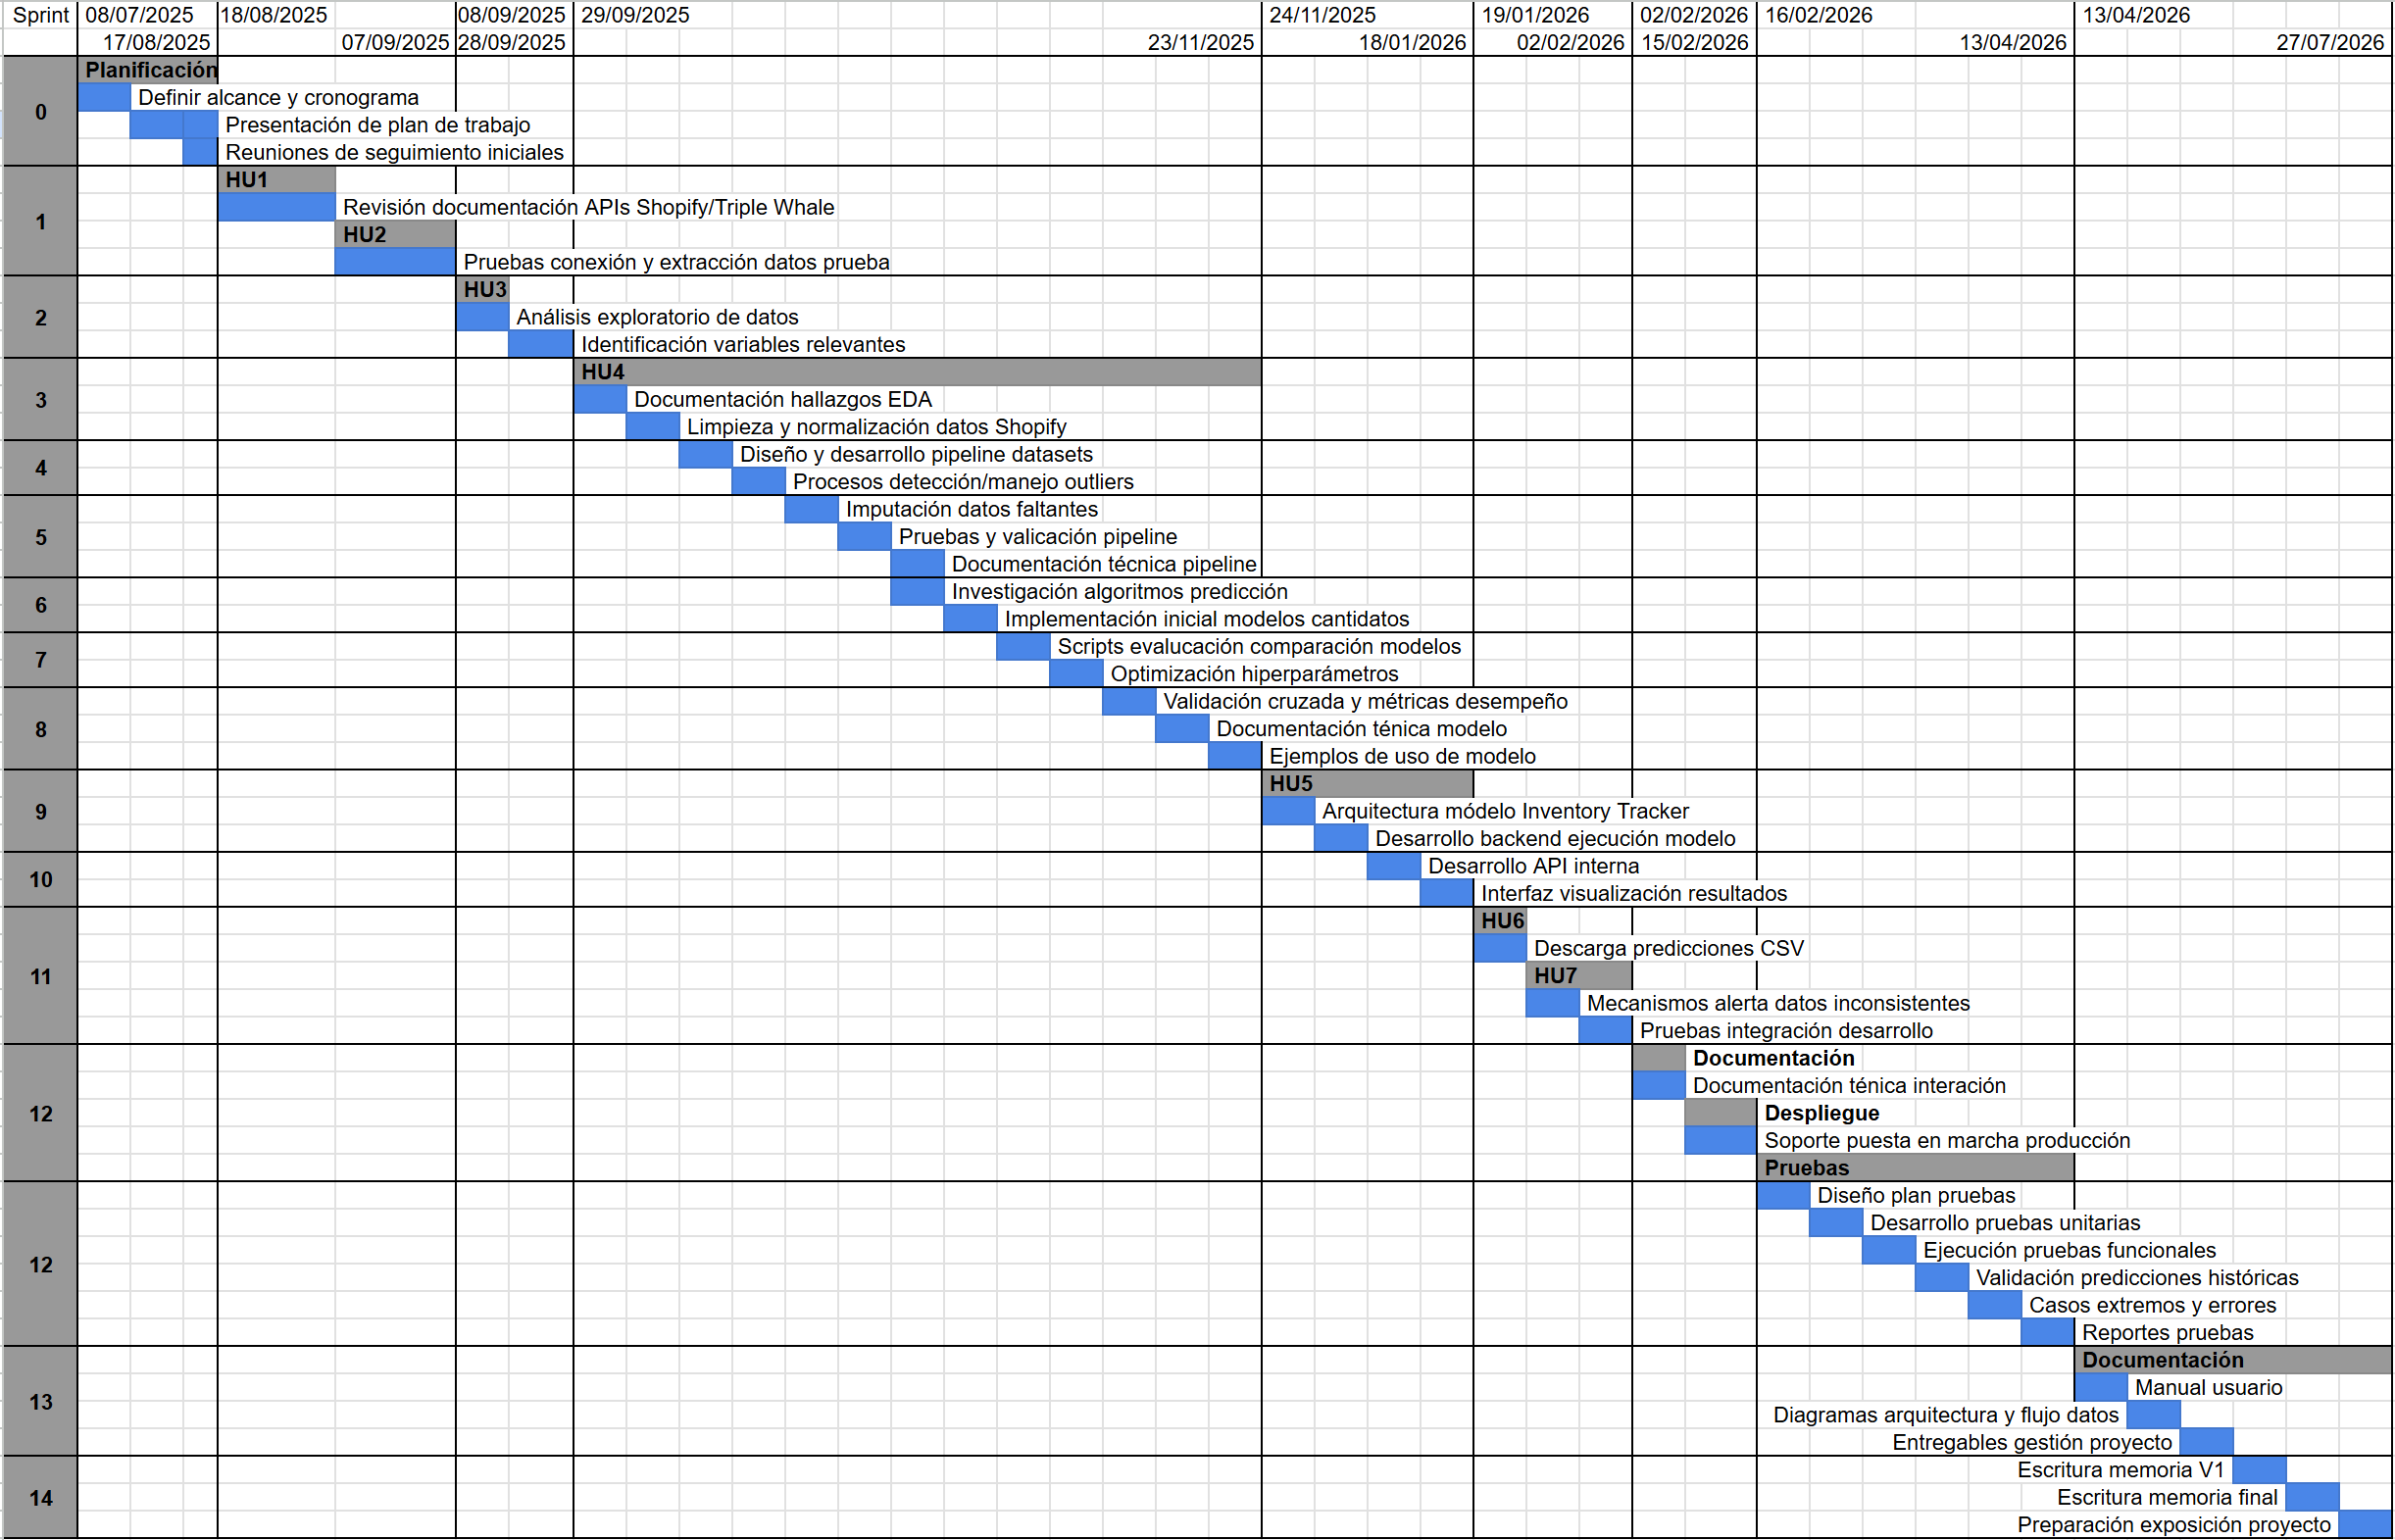
\includegraphics[width=1\textwidth]{./Figuras/Gantt-2.png}
\caption{Diagrama Gantt.}

\end{figure}



\section{12. Normativa y cumplimiento de datos (gobernanza)}


Los datos que se utilizarán en este proyecto contendrán identificadores únicos de usuarios obtenidos mediante una API privada de Shopify autorizada por la empresa cliente. El acceso será provisto exclusivamente con fines académicos y de desarrollo, y se realizará de acuerdo con los Términos de Servicio de Shopify.

Se tomarán medidas de ofuscación para evitar la exposición de información sensible, eliminando o codificando los datos identificables antes de su análisis o documentación. Asimismo, se aplicará el principio de minimización de datos, solicitando únicamente la información estrictamente necesaria para el desarrollo del modelo de predicción.

El uso de estos datos estará restringido por la Ley 25.326 de Protección de Datos Personales en Argentina y se prohibirá su difusión, redistribución o reutilización con otros fines. Además, se garantizarán condiciones de confidencialidad, evitando su publicación en reportes, repositorios o cualquier medio accesible a terceros no autorizados.

Estas acciones permitirán asegurar el cumplimiento normativo, la ética en el tratamiento de los datos y la protección de los derechos de los usuarios involucrados.



\section{13. Gestión de riesgos}
\label{sec:riesgos}


Riesgo 1: Baja calidad o inconsistencia de los datos obtenidos desde las APIs
\begin{itemize}
\item Severidad (S): 8
Una baja calidad en los datos afectaría directamente la precisión del modelo de predicción, comprometiendo la utilidad del sistema para la toma de decisiones.

\item Ocurrencia (O): 6
Aunque las \textit{APIs} de Shopify y Triple Whale son robustas, pueden presentarse inconsistencias o errores de carga en ciertos períodos, sobre todo en integraciones recientes.
\end{itemize}

Riesgo 2: Cambios en las \textit{APIs} externas

\begin{itemize}
\item Severidad (S): 7
Si se modifican los endpoints o se restringe el acceso a ciertas métricas, se vería afectada la actualización de datos históricos y la operación del sistema.

\item Ocurrencia (O): 5
Este tipo de cambios no son frecuentes, pero pueden ocurrir sin previo aviso por decisión unilateral de los proveedores.
\end{itemize}

Riesgo 3: Sobreajuste del modelo (\textit{overfitting})

\begin{itemize}
\item Severidad (S): 6
Si el modelo se ajusta demasiado a los datos históricos, podría perder capacidad de generalización, resultando en malas predicciones a futuro.

\item Ocurrencia (O): 5
Es un riesgo habitual en proyectos de \textit{machine learning}, aunque puede mitigarse con técnicas adecuadas de validación cruzada.
\end{itemize}

Riesgo 4: Incumplimiento del cronograma por complejidad técnica

\begin{itemize}
\item Severidad (S): 5
Un retraso significativo afectaría los tiempos de entrega al cliente y la integración con otros sistemas.

\item Ocurrencia (O): 7
Dada la complejidad de integrar varias fuentes y construir un modelo robusto, es un riesgo relevante.
\end{itemize}

Riesgo 5: Filtración o uso indebido de datos sensibles

\begin{itemize}
\item Severidad (S): 9
La exposición de datos identificables como correos electrónicos podría implicar consecuencias legales o de reputación graves.

\item Ocurrencia (O): 3
El riesgo es bajo ya que se prevé la implementación de medidas de ofuscación y restricciones de acceso.
\end{itemize}

Riesgo 6: Pérdida del vínculo laboral con la empresa cliente durante el desarrollo del proyecto

Justificación:
Existe la posibilidad de que durante el desarrollo del trabajo final se disuelva el vínculo laboral actual con la empresa \empclientename. En ese caso, se podría dificultar el acceso a datos, herramientas o validaciones necesarias para completar el proyecto, afectando su continuidad.

\begin{itemize}
	\item Severidad (S): 9
	La pérdida del acceso a recursos o información crítica podría implicar la necesidad de replantear partes sustanciales del proyecto o incluso buscar un nuevo cliente.
	\item Ocurrencia (O): 4
	Aunque actualmente el vínculo es estable, no puede descartarse completamente un cambio de situación laboral.
\end{itemize}

b) Tabla de gestión de riesgos      (El RPN se calcula como RPN=SxO)


Criterio adoptado:
Se tomarán medidas de mitigación para aquellos riesgos cuyo RPN supere los 30 puntos.


\begin{table}[htpb]
\centering
\begin{tabularx}{\linewidth}{@{}|X|c|c|c|c|c|c|@{}}
\hline
\rowcolor[HTML]{C0C0C0} 
Riesgo & S & O & RPN & S* & O* & RPN* \\ \hline
Baja calidad de datos       & 8  & 6  & 48    & 6   & 4   & 24     \\ \hline
Cambios en las APIs       & 7  & 5  & 35    & 6   & 3   & 18     \\ \hline
Sobreajuste del modelo       & 6  & 5  & 30    & 4   & 3   & 12     \\ \hline
Demoras en cronograma       & 5  & 7  & 35    & 3   & 4   & 12     \\ \hline
Filtración de datos       & 9  & 3  & 27    & 4   & 2   & 8     \\ \hline
Desvinculación laboral     & 9  & 4  & 36    & 4   & 2   & 8     \\ \hline
\end{tabularx}%
\end{table}

c) Plan de mitigación de riesgos

Riesgo 1: Baja calidad de datos

Plan de mitigación:
Se establecerán rutinas automáticas de validación y limpieza de datos antes de ser procesados por el modelo.

\begin{itemize}
\item Severidad (S): 6*
La calidad seguirá siendo importante, pero con validación previa se reduce su impacto.

\item Ocurrencia (O): 4*
La verificación regular reducirá las inconsistencias.
\end{itemize}


Riesgo 2: Cambios en las APIs

Plan de mitigación:
Se desarrollarán capas intermedias (\textit{wrappers}) para desacoplar el sistema de los cambios en las \textit{APIs}. Además, se monitorearán las actualizaciones oficiales.

\begin{itemize}
\item Severidad (S): 6*
Los cambios seguirán siendo relevantes, pero se reducirá su impacto directo.

\item Ocurrencia (O): 3*
La supervisión reduce la probabilidad de fallos inesperados.
\end{itemize}

Riesgo 4: Demoras en el cronograma

Plan de mitigación:
Se trabajará en ciclos iterativos con entregas parciales, priorizando funcionalidades clave para asegurar un producto mínimo viable en tiempo.

\begin{itemize}
\item Severidad (S): 3*
Las demoras parciales no afectarán el objetivo final.

\item Ocurrencia (O): 4*
La planificación iterativa mejora el control del avance.
\end{itemize}

Riesgo 6: Desvinculación laboral

Plan de mitigación:

Se acordará con la empresa la continuidad del acceso a los datos y a las herramientas necesarias para completar el trabajo final, aún en el caso de que se termine la relación laboral. Esto podría contemplarse en un documento formal o compromiso verbal con respaldo escrito.

\begin{itemize}
	\item Severidad (S): 4*
Si se garantiza el acceso a los recursos clave, el impacto se reduce notablemente.

	\item Ocurrencia (O): 2*
Al prever esta situación y dejarla documentada, disminuye la probabilidad de que se interrumpa el acceso al entorno de trabajo.
\end{itemize}


\begin{consigna}{red}
a) Identificación de los riesgos (al menos cinco) y estimación de sus consecuencias:
 
Riesgo 1: detallar el riesgo (riesgo es algo que si ocurre altera los planes previstos de forma negativa)
\begin{itemize}
	\item Severidad (S): mientras más severo, más alto es el número (usar números del 1 al 10).\\
	Justificar el motivo por el cual se asigna determinado número de severidad (S).
	\item Probabilidad de ocurrencia (O): mientras más probable, más alto es el número (usar del 1 al 10).\\
	Justificar el motivo por el cual se asigna determinado número de (O). 
\end{itemize}   

Riesgo 2:
\begin{itemize}
	\item Severidad (S): X.\\
	Justificación...
	\item Ocurrencia (O): Y.\\
	Justificación...
\end{itemize}

Riesgo 3:
\begin{itemize}
	\item Severidad (S):  X.\\
	Justificación...
	\item Ocurrencia (O): Y.\\
	Justificación...
\end{itemize}


b) Tabla de gestión de riesgos:      (El RPN se calcula como RPN=SxO)

\begin{table}[htpb]
\centering
\begin{tabularx}{\linewidth}{@{}|X|c|c|c|c|c|c|@{}}
\hline
\rowcolor[HTML]{C0C0C0} 
Riesgo & S & O & RPN & S* & O* & RPN* \\ \hline
       &   &   &     &    &    &      \\ \hline
       &   &   &     &    &    &      \\ \hline
       &   &   &     &    &    &      \\ \hline
       &   &   &     &    &    &      \\ \hline
       &   &   &     &    &    &      \\ \hline
\end{tabularx}%
\end{table}

Criterio adoptado: 

Se tomarán medidas de mitigación en los riesgos cuyos números de RPN sean mayores a...

Nota: los valores marcados con (*) en la tabla corresponden luego de haber aplicado la mitigación.

c) Plan de mitigación de los riesgos que originalmente excedían el RPN máximo establecido:
 
Riesgo 1: plan de mitigación (si por el RPN fuera necesario elaborar un plan de mitigación).
  Nueva asignación de S y O, con su respectiva justificación:
  \begin{itemize}
	\item Severidad (S*): mientras más severo, más alto es el número (usar números del 1 al 10).
          Justificar el motivo por el cual se asigna determinado número de severidad (S).
	\item Probabilidad de ocurrencia (O*): mientras más probable, más alto es el número (usar del 1 al 10).
          Justificar el motivo por el cual se asigna determinado número de (O).
	\end{itemize}

Riesgo 2: plan de mitigación (si por el RPN fuera necesario elaborar un plan de mitigación).
 
Riesgo 3: plan de mitigación (si por el RPN fuera necesario elaborar un plan de mitigación).

\end{consigna}

\section{14. Sprint Review}
\label{sec:sprint_review}

La revisión de sprint (\emph{Sprint Review}) es una práctica fundamental en metodologías ágiles. Consiste en revisar y evaluar lo que se ha completado al finalizar un sprint. En esta instancia, se presentan los avances y se verifica si las funcionalidades cumplen con los criterios de aceptación establecidos. También se identifican entregables parciales y se consideran ajustes si es necesario.

Aunque el proyecto aún se encuentre en etapa de planificación, esta sección permite proyectar cómo se evaluarán las funcionalidades más importantes del backlog. Esta mirada anticipada favorece la planificación enfocada en valor y permite reflexionar sobre posibles obstáculos.

\textbf{Objetivo:} anticipar cómo se evaluará el avance del proyecto a medida que se desarrollen las funcionalidades, utilizando como base al menos cuatro historias de usuario del \emph{Product Backlog}.


Seleccionar al menos 4 HU del Product Backlog. Para cada una, completar la siguiente tabla de revisión proyectada:

\textbf{Formato sugerido:}
\begin{table}[htpb]
\renewcommand{\arraystretch}{1.5}
\begin{tabular}{|>{\raggedright\arraybackslash}m{2.5cm}|
                >{\raggedright\arraybackslash}m{2.3cm}|
                >{\raggedright\arraybackslash}m{3cm}|
                >{\raggedright\arraybackslash}m{3cm}|
                >{\raggedright\arraybackslash}m{3cm}|}
\hline
\rowcolor[HTML]{CCCCCC}
\textbf{HU seleccionada} & \textbf{Tareas asociadas} & \textbf{Entregable esperado} & \textbf{¿Cómo sabrás que está cumplida?} & \textbf{Observaciones o riesgos} \\
\hline
                         & Tarea 1 &                             &                                           &                                     \\ \cline{2-2}
\multirow{-2}{=}{HU1}    & Tarea 2 & \multirow{-2}{=}{Módulo funcional} & \multirow{-2}{=}{Cumple criterios de aceptación definidos} & \multirow{-2}{=}{Falta validar con el tutor} \\
\hline
                         & Tarea 1 &                             &                                           &                                     \\ \cline{2-2}
\multirow{-2}{=}{HU3}    & Tarea 2 & \multirow{-2}{=}{Reporte generado} & \multirow{-2}{=}{Exportación disponible y clara} & \multirow{-2}{=}{Requiere datos reales} \\
\hline
                         & Tarea 1 &                             &                                           &                                     \\ \cline{2-2}
\multirow{-2}{=}{HU5}    & Tarea 2 & \multirow{-2}{=}{Panel de gestión} & \multirow{-2}{=}{Roles diferenciados operativos} & \multirow{-2}{=}{Riesgo en integración} \\
\hline
                         & Tarea 1 &                             &                                           &                                     \\ \cline{2-2}
\multirow{-2}{=}{HU7}    & Tarea 2 & \multirow{-2}{=}{Informe trimestral} & \multirow{-2}{=}{PDF con gráficos y evolución} & \multirow{-2}{=}{Puede faltar tiempo para ajustes} \\
\hline
\end{tabular}
\end{table}

\section{15. Sprint Retrospective}    
\label{sec:sprint_retro}

La retrospectiva de sprint es una práctica orientada a la mejora continua. Al finalizar un sprint, el equipo (o el alumno, si trabaja de forma individual) reflexiona sobre lo que funcionó bien, lo que puede mejorarse y qué acciones concretas pueden implementarse para trabajar mejor en el futuro.

Durante la cursada se propuso el uso de la \textbf{Estrella de la Retrospectiva}, que organiza la reflexión en torno a cinco ejes:

\begin{itemize}
\item  ¿Qué hacer más?
\item  ¿Qué hacer menos?
\item  ¿Qué mantener?
\item  ¿Qué empezar a hacer?
\item  ¿Qué dejar de hacer?
\end{itemize}

Aun en una etapa temprana, esta herramienta permite que el alumno planifique su forma de trabajar, identifique anticipadamente posibles dificultades y diseñe estrategias de organización personal.

\textbf{Objetivo:} reflexionar sobre las condiciones iniciales del proyecto, identificando fortalezas, posibles dificultades y estrategias de mejora, incluso antes del inicio del desarrollo.


Completar la siguiente tabla tomando como referencia los cinco ejes de la Estrella de la Retrospectiva (\emph{Starfish} o estrella de mar). Esta instancia te ayudará a definir buenas prácticas desde el inicio y prepararte para enfrentar el trabajo de forma organizada y flexible. Se deberá completar la tabla al menos para 3 sprints técnicos y 1 no técnico.

\textbf{Formato sugerido:}

\begin{table}[htpb]
\renewcommand{\arraystretch}{1.4}
\begin{tabular}{|>{\raggedright\arraybackslash}p{1.8cm}|
                >{\raggedright\arraybackslash}p{2.3cm}|
                >{\raggedright\arraybackslash}p{2.3cm}|
                >{\raggedright\arraybackslash}p{2.3cm}|
                >{\raggedright\arraybackslash}p{2.3cm}|
                >{\raggedright\arraybackslash}p{2.3cm}|}
\hline
\rowcolor[HTML]{CCCCCC} 
\textbf{Sprint tipo y N°} & \textbf{¿Qué hacer más?} & \textbf{¿Qué hacer menos?} & \textbf{¿Qué mantener?} & \textbf{¿Qué empezar a hacer?} & \textbf{¿Qué dejar de hacer?} \\
\hline
Sprint técnico - 1 & Validaciones continuas con el alumno & Cambios sin versión registrada & Pruebas con datos simulados & Documentar cambios propuestos & Ajustes sin análisis de impacto \\
\hline
Sprint técnico - 2 & Verificar configuraciones en múltiples escenarios & Modificar parámetros sin guardar historial & Perfiles reutilizables & Usar logs para configuración & Repetir pruebas manuales innecesarias \\
\hline
Sprint técnico - 8 & Comparar correlaciones con casos previos & Cambiar parámetros sin justificar & Revisión cruzada de métricas & Anotar configuraciones usadas & Trabajar sin respaldo de datos \\
\hline
Sprint no técnico - 12 (por ej.: ``Defensa'') & Ensayos orales con feedback & Cambiar contenidos en la memoria & Material visual claro & Dividir la presentación por bloques & Agregar gráficos difíciles de explicar \\
\hline
\end{tabular}
\end{table}




\end{document}